\documentclass{beamer}
\usepackage{hyperref}


\usetheme{Copenhagen}



\newcommand{\github}{
\href{https://github.com/A-M-Kharazi/Machine-Learning-TMU}{GitHub}
}

\definecolor{links}{HTML}{2A1B81}
\hypersetup{colorlinks,linkcolor=,urlcolor=links}


\title{Wavelet Transform}
\subtitle{Machine Learning}
\author{Amir Mohammad Kharazi}
\institute{Tarbiat Modares University\\\vspace{10mm}
\github
}

\date{2022}




\newtheorem{solu}{Solution}
\newtheorem{thatis}{That is :}


\begin{document}

	
	
	
	\frame {
		\titlepage
	}
	\frame {
		\frametitle{Table of Contents}
		\tableofcontents
	}
	
	\section{Signal Processing}
	\begin{frame}
		\frametitle{Signals vs Time Series}
		
		\begin{itemize}
			\item
			In a time-series data set, the to-be-predicted value ($y$) is a function of time ($y = y(t)$).
			
			\item
			
			A signal is a more general version of this where the dependent variable $y$ does not have to be a function of time ($y = y(t)$);  it can be a function of spatial coordinates ($y = y(x, y)$), distance from the source ( $y = y(r)$ ), etc. 
			
		\end{itemize}	
	\end{frame}
	
	\begin{frame}
		\frametitle{Signals}
		\begin{itemize}
			\item
			
			 Signals can come in many different forms and shapes: you can think of audio signals, pictures, video signals, geophysical signals (seismic data), sonar and radar data and medical signals (EEG, ECG, EMG).
			
		\end{itemize}


		
		
	\end{frame}
	
	\begin{frame}
		\frametitle{Time Signals}
		
		\begin{itemize}
			\item 
			Continuous time-domain ( Most of real Signals ) - Analog
			\item
			Discrete-time domain ( Digitized version )
		\end{itemize}

	\end{frame}
	
	\begin{frame}
		\frametitle{Digitizing an analog signal}
		
		\begin{itemize}
			\item 
			Is done by sampling it with a specific sampling rate
			
			\item 
			
			Under-Sampled ( aliasing and the wagon-wheel effect )
			
			\item
			
			 Nyquist rate : twice the highest frequency present in the signal
			 
			 \item
			 
			 To prevent under-sampling, usually a frequency much higher than the Nyquist rate is chosen as the sampling frequency.
			
		\end{itemize}

	\end{frame}

	\begin{frame}
		\frametitle{Digitizing an analog signal}
		
		\begin{center}
			\begin{figure}\label{fig1}
				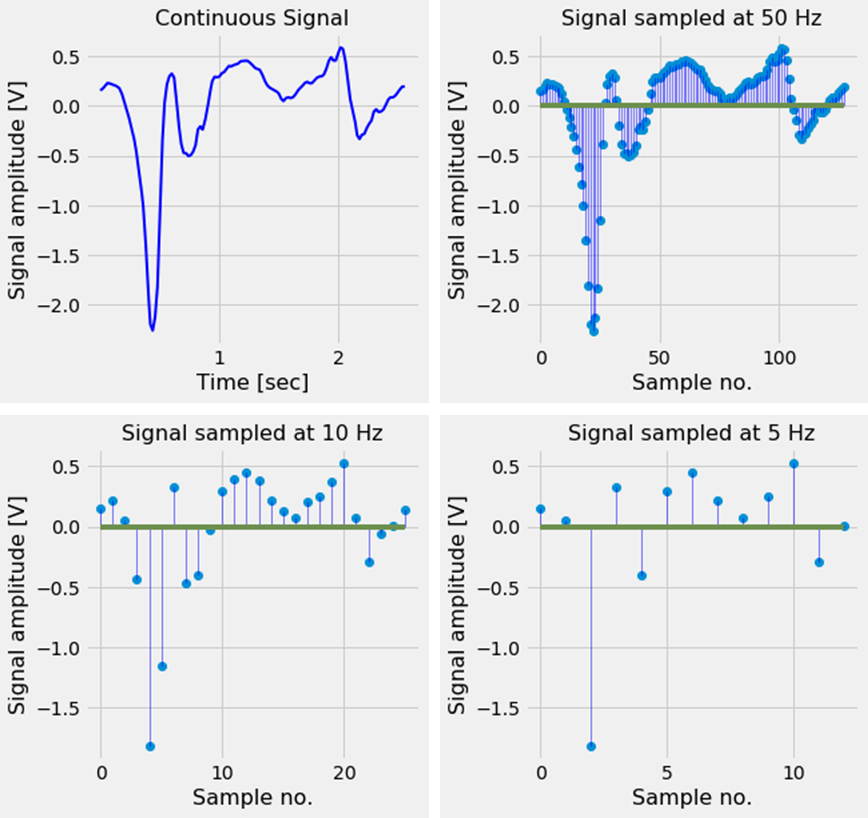
\includegraphics[scale=0.27]{continious_signal_samples.png}
				\caption{A continuous signal sampled at different frequencies.}
			\end{figure}
		\end{center}

	\end{frame}

	\begin{frame}
		\frametitle{Periodic Signals}
		
		\begin{itemize}
			\item
			If the signal contains a pattern, which repeats itself after a specific period of time.
			
			\item
			The time it takes for an periodic signal to repeat itself is called the period $P$.
			
			\item
			The distance it travels in this period is called the wavelength $\lambda$
			
			\item
			The frequency $f$ is the inverse of the Period.
			
			\item
			$f = \frac{1}{P} = \frac{V}{\lambda}$
			
			
		\end{itemize}
		
		
	\end{frame}

	\section{Fourier Transform}
	\begin{frame}
		\frametitle{Fourier series}
		
		\begin{itemize}
			\item
			Is a sum that represents a periodic function as a sum of sine and cosine waves
			
		\end{itemize}
	
		\[
		S_N(x) = \frac{a_0}{2} + \sum\limits_{i=1}^{N}\left(a_i\cos\left(\frac{2\pi}{P}i x\right) + b_i \sin\left(\frac{2\pi}{P}i x\right)\right)
		\]
			
	\end{frame}

	\begin{frame}
		\frametitle{Fourier Transform}
		
		\begin{itemize}
			\item
			
			Every signal, no matter how complex it looks, can be decomposed into a sum of its simpler signals.
			
			\item
			These simpler signals are trigonometric functions (sine and cosine waves).
			
			\item
			
			Transform a signal from its time-domain to its frequency domain.
			
		\end{itemize}
		
	\end{frame}

	\begin{frame}
		\frametitle{Example}
		\begin{itemize}
			\item 
			We have five sine-waves (blue signals)
			\item
			By combining these signals we form a new composite signal (black)
			\item
			 The Fourier Transform transforms this signal to the frequency-domain (red signal) and shows us at which frequencies the component signals oscillate.
			 
			 \item Code is available at \github
			
		\end{itemize}
		
	\end{frame}
	
	\begin{frame}
		\frametitle{Example}
		\begin{center}
			\begin{figure}\label{fig2}
				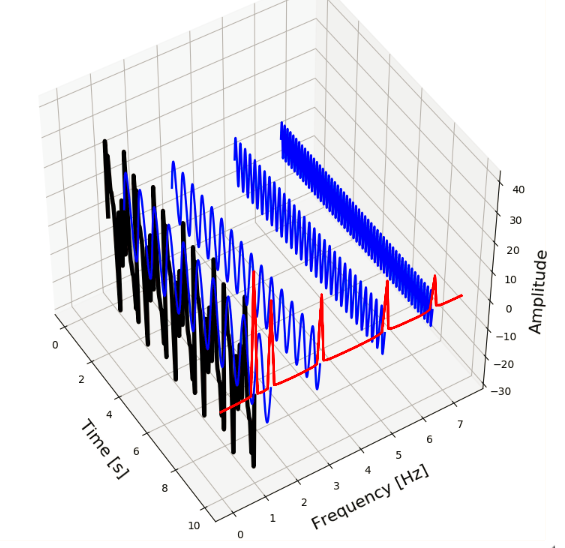
\includegraphics[scale=0.37]{signals3D_4.png}
				\caption{ A signal (black) consisting of multiple component signals (blue) with DFT (red).}
			\end{figure}
		\end{center}
	\end{frame}

	\begin{frame}
		\frametitle{FFT}
		\begin{itemize}
			\item 
			FFT stands for Fast Fourier Transform.
			
			\item
			In python FFT can be calculated using Scipy.
			
			\item
			If for example,  our signal is sampled at a rate $f_s$ of $100 Hz$.The FFT will return the frequency spectrum up to a frequency of $f_s / 2 = 50 Hz$.

			
			\item
			
			The higher your sampling rate is, the higher the maximum frequency is FFT can calculate.
			
		\end{itemize}
	\end{frame}
	
	\begin{frame}
		\frametitle{Example}
		
		Code is available at \github.
		
		\begin{center}
			\begin{figure}\label{fig3}
				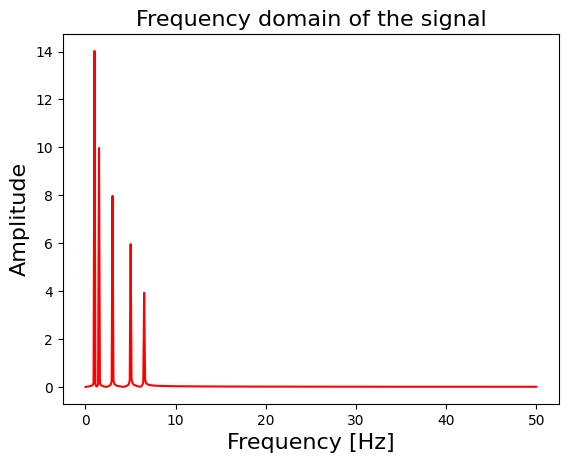
\includegraphics[scale=0.45]{fft_of_signal.png}
				\caption{Red signal from the previous example}
			\end{figure}
		\end{center}
		
	\end{frame}

	\subsection{Statistical parameter estimation and feature extraction}
	\begin{frame}
		\frametitle{Statistical parameter estimation and feature extraction}
		
		\begin{itemize}
			\item
			
			After we have transformed a signal to the frequency-domain, we can extract features from each of these transformed signals.
			
			\item
			
			Use these features as input in standard classifiers like Random Forest, Logistic Regression, Gradient Boosting or Support Vector Machines.
			
		\end{itemize}	
		
	\end{frame}

\begin{frame}
	\frametitle{Statistical parameter estimation and feature extraction}
		Which features can we extract from these transformations? 
	
	\begin{itemize}


		\item
		
		A good first step is the value of the frequencies at which oscillations occur and the corresponding amplitudes.
		
		\item
		
		In other words; the x and y-position of the peaks in the frequency spectrum.
	\end{itemize}
	
\end{frame}



\section{Wavelet}
\begin{frame}
	\frametitle{Summary of Fourier Transform}
	
	\begin{itemize}
		\item 
		 Transform a signal from its time-domain to its frequency domain
		
		\item
		
		 The peaks in the frequency spectrum indicate the most occurring frequencies in the signal
		
		
		\item
		The location (frequency-value) and height (amplitude) of the peaks in the frequency spectrum then can be used as input for Classifiers like Random Forest or Gradient Boosting

	\end{itemize}
	
\end{frame}

\begin{frame}
	\frametitle{Problem ? }
	
	\begin{itemize}
		\item 
			The general rule is that this approach of using the Fourier Transform will work very well when the frequency spectrum is stationary.
		
		\item
		
		That is, the frequencies present in the signal are not time-dependent; if a signal contains a frequency of $x$ $Hz$ this frequency should be present equally anywhere in the signal.
		
	\end{itemize}
	
\end{frame}


\begin{frame}
	\frametitle{Problem ?}
	
	\begin{itemize}
		\item
		The more non-stationary/dynamic a signal is, the worse the results will be.
		
		\item
		That’s too bad, since most of the signals we see in real life are non-stationary in nature.
		
	\end{itemize}


	\begin{solu}
		A much better approach for analyzing dynamic signals is to use the Wavelet Transform instead of the Fourier Transform.
	\end{solu}

\end{frame}

\begin{frame}
	\frametitle{Example}
	
	\begin{itemize}
		\item 
		The thing about the Fourier Transform is that it has a high resolution in the frequency-domain but zero resolution in the time-domain.
		
		\item
		
		This means that it can tell us exactly which frequencies are present in a signal, but not at which location in time these frequencies have occurred.
		
		\item 
		Code is available at \github
		
	\end{itemize}
	
\end{frame}


\begin{frame}
	\frametitle{Example}
	\begin{center}
		\begin{figure}\label{fig4}
			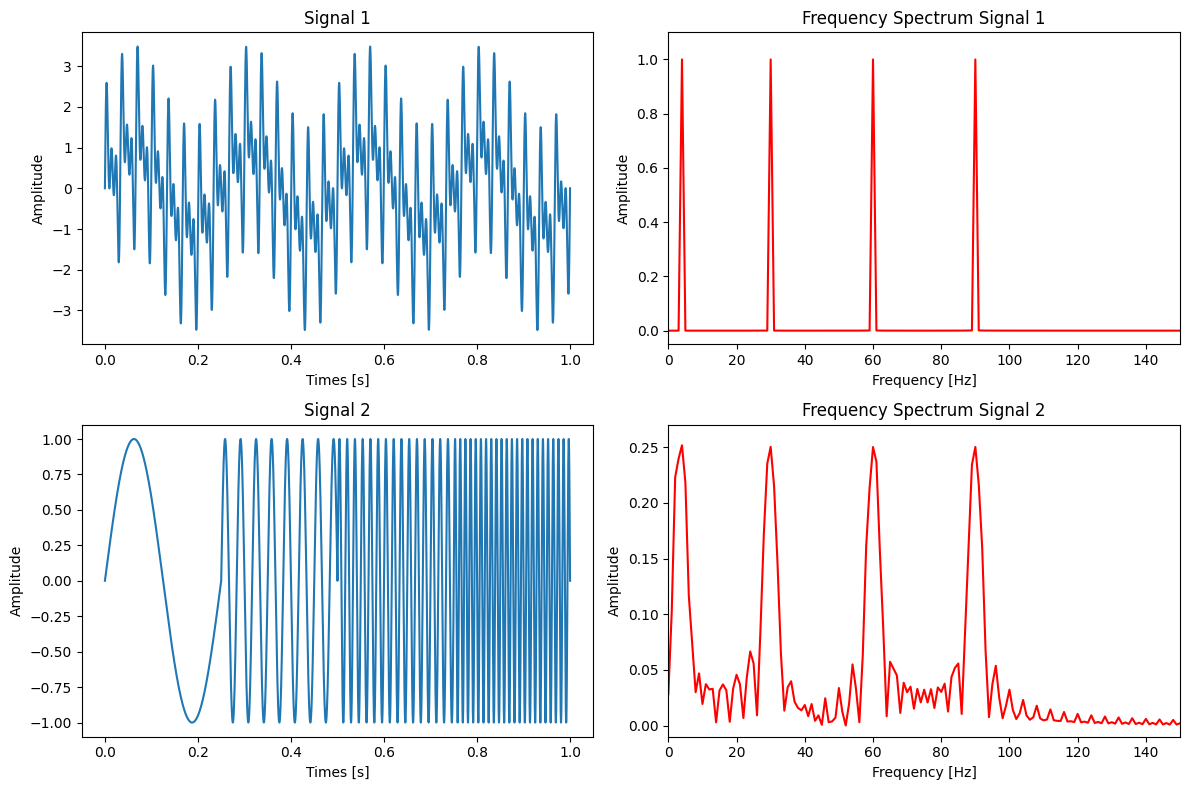
\includegraphics[scale=0.25]{fft_spectra-1.png}
			\caption{ The signals and frequency spectrum of a signal which contains four frequencies at all times (top), four different frequencies at four different times (bottom).}	
		\end{figure}
	\end{center}
	
	
\end{frame}


\subsection{Short-Time Fourier Transform}
\begin{frame}
	\frametitle{From Fourier Transform to Wavelet Transform}
	\framesubtitle{Short-Time Fourier Transform.}
	
	\begin{itemize}
		\item
		Original signal is splitted into several parts of equal length (which may or may not have an overlap)
		
		\item
		How  ? by using a sliding window before applying the Fourier Transform.
		
		\item
		
		if we split our signal into 10 parts, and the Fourier Transform detects a specific frequency in the second part,
		
		\item
		
		then we know for sure that this frequency has occurred between $\frac{2}{10}$th and $\frac{3}{10}$th of our original signal.
		
		
	\end{itemize}
\end{frame}

\begin{frame}
	\frametitle{From Fourier Transform to Wavelet Transform}
	\framesubtitle{Short-Time Fourier Transform.}
	The main problem with this approach is that you run into the theoretical limits of the Fourier Transform known as the uncertainty principle.
	\begin{thatis}
		The smaller we make the size of the window the more we will know about where a frequency has occurred in the signal, but less about the frequency value itself. The larger we make the size of the window the more we will know about the frequency value and less about the time.
	\end{thatis}
	
\end{frame}


\subsection{Wavelet Transform}
\begin{frame}
	\frametitle{Wavelet Transform}
	
	\begin{itemize}
		\item
		A better approach for analyzing signals with a dynamical frequency spectrum is the Wavelet Transform.
		\item
		The Wavelet Transform has a high resolution in both the frequency- and the time-domain. It does not only tell us which frequencies are present in a signal, but also at which time these frequencies have occurred.
		
		\item
		This is accomplished by working with different scales. First we look at the signal with a large scale/window and analyze ‘large’ features and then we look at the signal with smaller scales in order to analyze smaller features.
		
		
	\end{itemize}

\end{frame}



\begin{frame}
	\frametitle{TS vs FT vs Short-Time FT vs Wavelet}
	\begin{center}
		\begin{figure}\label{fig5}
			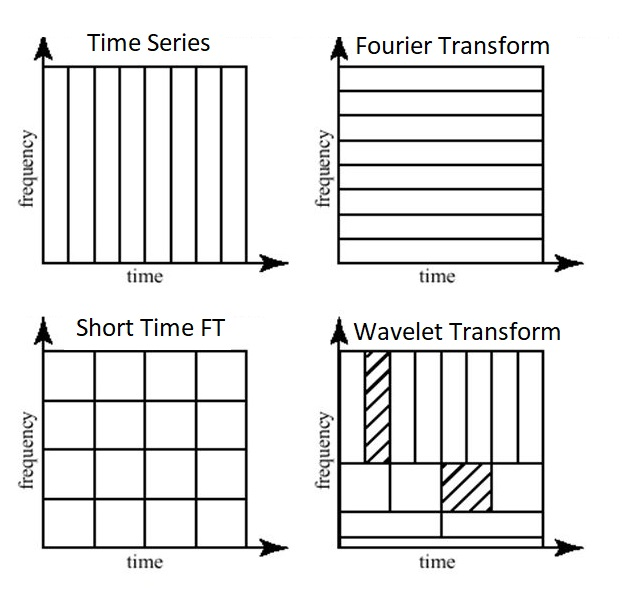
\includegraphics[scale=0.27]{Comparisonoftransformations.jpg}
			\caption{A schematic overview of the time and frequency resolutions of the different transformations in comparison with the original time-series dataset. The size and orientations of the block gives an indication of the resolution size.}
		\end{figure}
	\end{center}

\end{frame}

\begin{frame}
	\frametitle{Wavelet Transform }
	The Wavelet Transform has:
	
	\begin{itemize}
		\item 
		For small frequency values a high resolution in the frequency domain, low resolution in the time- domain,
		
		\item
		
		For large frequency values a low resolution in the frequency domain, high resolution in the time domain.
		
	\end{itemize}

\end{frame}


\begin{frame}
	\frametitle{Wavelet Transform}
	
	In other words, the Wavelet Transforms makes a trade-off; at scales in which time-dependent features are interesting it has a high resolution in the time-domain and at scales in which frequency-dependent features are interesting it has a high resolution in the frequency domain.
	
	
	
\end{frame}

\begin{frame}
	\frametitle{How does the Wavelet Transform work?}
	\begin{itemize}
		\item
		The Fourier Transform uses a series of sine-waves with different frequencies to analyze a signal. That is, a signal is represented through a linear combination of sine-waves.
		
		\item
		
		The Wavelet Transform uses a series of functions called wavelets, each with a different scale.
		
	\end{itemize}
	
\end{frame}


\begin{frame}
	\frametitle{How does the Wavelet Transform work?}
	The word wavelet means a small wave, and this is exactly what a wavelet is.
	\begin{center}
		\begin{figure}\label{fig6}
			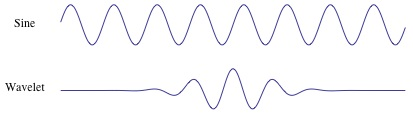
\includegraphics[scale=0.5]{Wavelet-Out1.jpg}
			\caption{ The difference between a sine-wave and a Wavelet. The sine-wave is infinitely long and the Wavelet is localized in time.}
		\end{figure}
	\end{center}
	
\end{frame}

\begin{frame}
	\frametitle{How does the Wavelet Transform work?}
	
	\begin{itemize}
		\item
		 The main difference is that the sine-wave is not localized in time
		
		\item
		
		A wavelet is localized in time, which allows the wavelet transform to obtain time-information in addition to frequency information
		
	\end{itemize}

\end{frame}

\begin{frame}
	\frametitle{The different types of Wavelet families}
	
	\begin{itemize}
		\item
			Another difference between the Fourier Transform and the Wavelet Transform is that there are many different families (types) of wavelets.
		
		\item
		
		This means that we can choose a specific wavelet family which fits best with the features we are looking for in our signal.
		
		\item Check the code at \github.
	\end{itemize}
	

\end{frame}


\begin{frame}
	\frametitle{Wavelet families}
	\begin{center}
			\begin{figure}\label{fig7}
			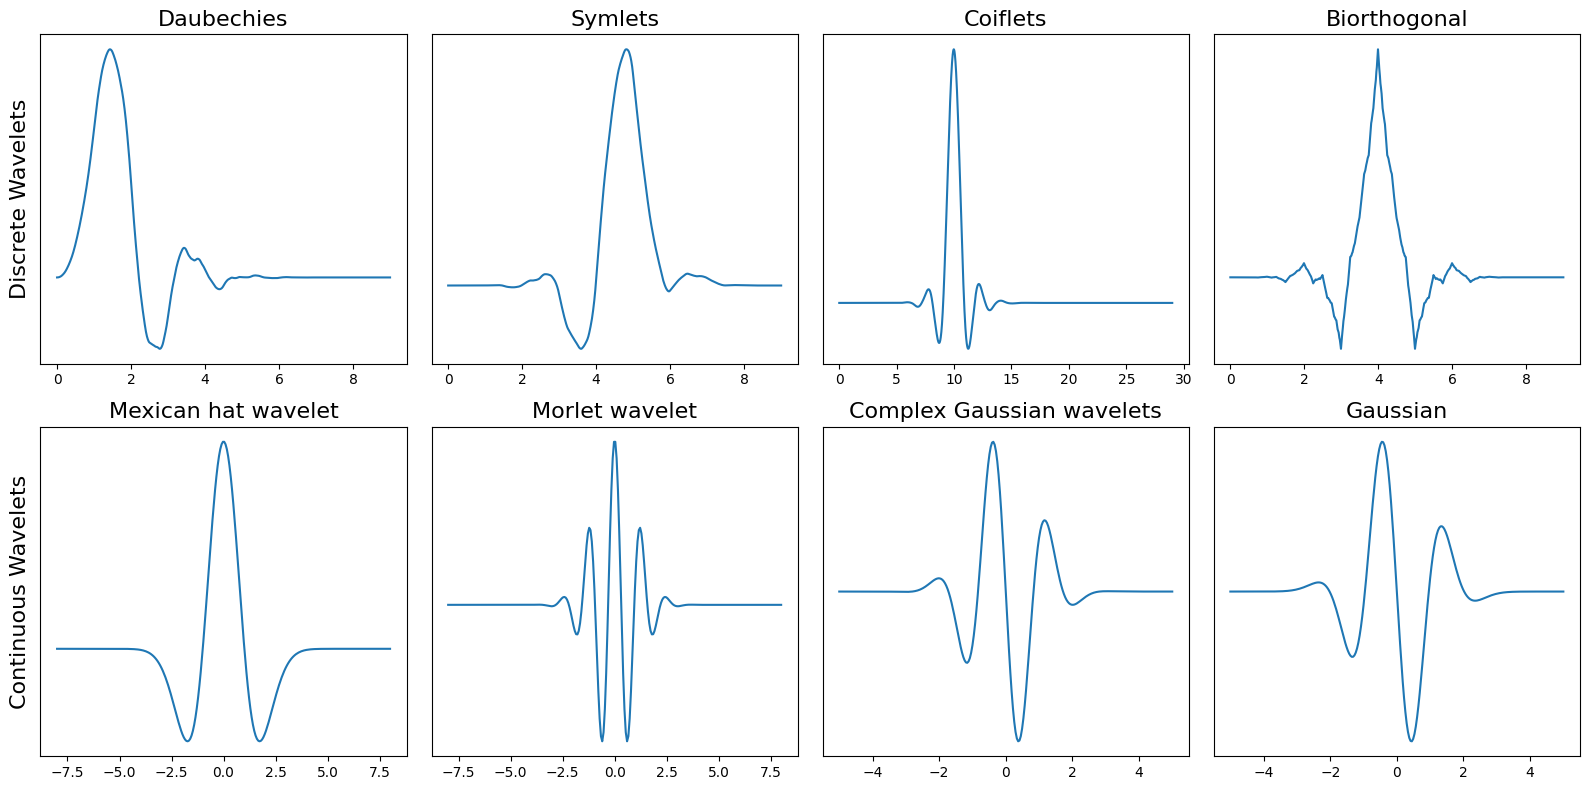
\includegraphics[scale=0.25]{wavelet_families.png}
			\caption{ Several families of Wavelets. In the first row we see discrete wavelets and in the second row we see several continuous wavelets.}
		\end{figure}
	\end{center}
	
\end{frame}


\begin{frame}
	\frametitle{A wavelet must have}
	
	\begin{enumerate}
		\item
		 finite energy : Means that it is localized in time and frequency; it is integrable and the inner product between the wavelet and the signal always exists.
		\item
		zero mean : 
		
		Wavelet has zero mean in the time-domain, a zero at zero frequency in the time-domain. This is necessary to ensure that it is integrable and the inverse of the wavelet transform can also be calculated.
		
	\end{enumerate}
	
\end{frame}

\begin{frame}
	\frametitle{Continuous Wavelet Transform}
	
	
	\[
	X_w(a,b) = \frac{1}{\sqrt{|a|}}\int\limits_{-\infty}^{+\infty}x(t)
	\bar{\psi}\left(\frac{t-b}{a}\right)dt
	\]
	
	\begin{itemize}
		\item 
		where $\psi(t)$ is the continuous mother wavelet which gets scaled by a factor of $a$ and translated by a factor of $b$. 
		\item
		The values of the scaling and translation factors are continuous,
		
		\item
		
		which means that there can be an infinite amount of wavelets. You can scale the mother wavelet with a factor of $1.3$, or $1.31$, and $1.311$, and $1.3111$, etc.
		
	\end{itemize}
	
\end{frame}

\begin{frame}
	\frametitle{Discrete Wavelet Transform}
	
	\begin{itemize}
		\item 
		the main difference is that the DWT uses discrete values for the scale and translation factor. 
		\item
		The scale factor increases in powers of two, so ( $a = 1, 2, 4, \dots$ ) and the translation factor increases integer values ( $b = 1, 2, 3, \dots$ ).
		\item
		
		\textbf{PS}:  The DWT is only discrete in the scale and translation domain, not in the time-domain. 
		
	\end{itemize}
	
\end{frame}

\begin{frame}
	\frametitle{Apply the DWT on a signal}
	
	\begin{itemize}
		\item
		We start with the smallest scale. As we have seen before, small scales correspond with high frequencies. This means that we first analyze high frequency behavior. 
		
		\item
		At the second stage, the scale increases with a factor of two (the frequency decreases with a factor of two), and we are analyzing behavior around half of the maximum frequency.
		
		\item
		
		At the third stage, the scale factor is four and we are analyzing frequency behavior around a quarter of the maximum frequency.
		
		\item
		
		And this goes on and on, until we have reached the maximum decomposition level.
	\end{itemize}
	
\end{frame}


\begin{frame}
	\frametitle{maximum decomposition level?}
	
	\begin{itemize}
		\item 
		we should  know that at each subsequent stage the number of samples in the signal is reduced with a factor of two. 
		
		\item
		
		At lower frequency values, you will need less samples to satisfy the Nyquist rate so there is no need to keep the higher number of samples in the signal
		
		\item
		
		Due to this downsampling, at some stage in the process the number of samples in our signal will become smaller than the length of the wavelet filter and we will have reached the maximum decomposition level.
		
	\end{itemize}
	
\end{frame}

\begin{frame}
	\frametitle{Example}
	Suppose we have a signal with frequencies up to $1000$ $Hz$
	
	\begin{itemize}
		\item
		In the first stage we split our signal into a low-frequency part and a high-frequency part. i.e. $0-500$ Hz and $500-1000$ $Hz$.
		\item
		At the second stage we take the low-frequency part and again split it into two parts: $0-250$ $Hz$ and $250-500$ $Hz$.
		\item
		At the third stage we split the $0-250$ $Hz$ part into a $0-125$ $Hz$ part and a $125-250$ $Hz$ part.
		This goes on until we have reached the level of refinement we need or until we run out of samples.
	
	\end{itemize}
	
	
\end{frame}

\begin{frame}
	\frametitle{Example}
	\begin{center}
		\begin{figure}\label{fig8}
			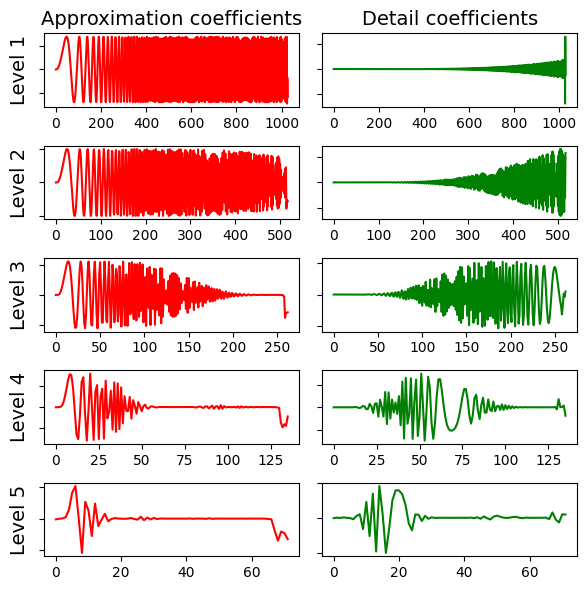
\includegraphics[scale=0.3]{multilevel_coefficients_schematic.png}
			\caption{The approximation and detail coefficients of the sym5 wavelet (level 1 to 5) applied on a chirp signal, from level 1 to 5. On the left we can see a schematic representation of the high pass and low pass filters applied on the signal at each level. available at \github.}
		\end{figure}
	\end{center}
\end{frame}


\begin{frame}
	\frametitle{Practical Example}
	
	Using the Continuous Wavelet Transform and a Convolutional Neural Network for classification of signals. Full detail at \github.
	
\end{frame}






	
	
\end{document}